\documentclass[10pt,twocolumn]{article}
\usepackage[margin=0.63in,columnsep=0.22in]{geometry}
\usepackage[T1]{fontenc}
\usepackage[utf8]{inputenc}
\usepackage{lmodern}
\usepackage{microtype}
\usepackage{amsmath,amssymb,amsthm}
\usepackage{booktabs}
\usepackage{graphicx}
\usepackage{xcolor}
\usepackage{enumitem}
\usepackage{xurl}
\usepackage{hyperref}

\hypersetup{
  colorlinks=true,
  linkcolor=blue!60!black,
  citecolor=blue!60!black,
  urlcolor=blue!60!black,
  pdftitle={Constructive Lean 4 Kernel and Exact-Rational Certificates for Google Research Cogentic Log-Rank Conjecture Proof},
  pdfauthor={Lluis Eriksson}
}

\newtheorem{proposition}{Proposition}
\newtheorem{definition}{Definition}
\newcommand{\QQ}{\mathbb{Q}}
\newcommand{\ZZ}{\mathbb{Z}}

\title{\vspace{-0.9em}\textbf{Constructive Lean~4 Kernel and Exact-Rational Certificates for Google Research Cogentic's $O(r^{1/2 - 5\times 10^{-6}})$ Log-Rank Conjecture Proof}}
\author{Lluis Eriksson\thanks{Independent Researcher. Code, Lean~4 proofs, and certificates: MIT License; manuscript and figures: CC-BY-4.0. Prepared with transparent AI coding, formalization, and drafting assistance via Google Antigravity; all Lean~4 theorems, exact-$\QQ$ verifiers, and adversarial tests were independently compiled and verified locally. Repository: \href{https://github.com/lluiseriksson/cogentic-logrank-certificates}{\nolinkurl{github.com/lluiseriksson/cogentic-logrank-certificates}}.}}
\date{November 25, 2026}

\begin{document}
\maketitle
\vspace{-1.2em}

\begin{abstract}
Google Research's Cogentic framework (Nov.~25, 2026) broke the $\sqrt{r}$ barrier for the Lov\'asz--Saks Log-Rank Conjecture, proving that every rank-$r$ Boolean matrix $M\in\{0,1\}^{X\times Y}$ has a monochromatic rectangle of density $\ge 2^{-C r^{1/2-\varepsilon}}$ and deterministic communication complexity $D_{\mathrm{cc}}(M) \le C' r^{1/2-\varepsilon}$ with $\varepsilon = 5\times 10^{-6}$, $C = 238$, and $C' = 750 C = 178{,}500$. We deliver an explicitly scoped, standalone, zero-floating-point verification stack for the deterministic algebraic, third-moment spectral-tensor, Bregman-divergence, monochromatic rank-split, and quantitative Nisan--Wigderson recursion pillars of this breakthrough. Layer~1 (\nolinkurl{CogenticLogRank.lean}) proves 18 constructive Lean~4.35.0 theorems (zero \texttt{sorry}, zero \texttt{axiom}, zero \texttt{Classical.choice}, zero warnings; 4 zero-axiom and 14 \texttt{[propext, Quot.sound]}) mechanizing Eq.~(1.6) pointwise Booleanity, the degree-1 AM--GM barrier vs.\ degree-2 $\cosh$-tilt $\lambda^2$-cancellation, Eq.~(1.7) variational penalty concavity/slope, scalar/eigenvalue Eq.~(2.2) Bregman nonnegativity, the $2\times 2$ commutator trace identity, inductive Lemma~2.1(1) leverage defect, universal 2D Hermite $c_2$ covariance, and every discrete step of Proposition~A.3 ($2^{11}<3^7$, $3\cdot 29^4<4\cdot 27^4$, rank-split $\lfloor 3k/4\rfloor$, $750 C_0$). Layer~2 (\nolinkurl{LOGRANK-COGENTIC-CERT-1.0}) is a pure-stdlib Python \texttt{Fraction} auditor across four modes that certifies 16 canonical witnesses in $0.099$--$16.937\,\mathrm{ms}$—including an exact isospectral separation between Boolean $S=J_4-2I_4$ ($E_3=3/2$, hollow slice energy $3/32$) and the Rademacher barrier $A_{\mathrm{Rad}}$ ($E_3=0$, hollow energy $0$)—and rejects 62/62 live adversarial forgeries with exact branch assertions (66/66 pytest checks).
\end{abstract}

\section{Introduction and Scope Calibration}\label{sec:intro}
Lov\'asz and Saks~\cite{lovasz1993lattices} conjectured that $D_{\mathrm{cc}}(M) \le (\log_2 \operatorname{rank}_{\mathbb{R}}(M))^{O(1)}$ for every Boolean matrix $M\in\{0,1\}^{X\times Y}$. Via Nisan--Wigderson rank-halving~\cite{nisan1995rank}, upper bounds progressed from $O(\sqrt{r}\log r)$~\cite{lovett2016communication} to $O(\sqrt{r})$~\cite{sudakov2025matrix}, where $\gamma_2$-norm and discrepancy methods hit a natural $\sqrt{r}$ barrier. On November~25, 2026, Google Research's Cogentic system~\cite{cogentic2026logrank,cai2026cogentic} proved Theorem~1.1: $D_{\mathrm{cc}}(M) \le 750\cdot 238\, r^{1/2-5\times 10^{-6}}$ by exploiting pointwise Booleanity $S(x,y)^2 = 1$ of the sign matrix $S = \pm(2M - J)$:
\begin{equation}
-2 s_1 u_1(x) v_1(y) A_\perp(x,y) = A_\perp(x,y)^2 + s_1^2 u_1(x)^2 v_1(y)^2 - 1,
\tag{1.6}\label{eq:eq16}
\end{equation}
where $S = s_1 u_1 v_1^\top + \sum_{k=1}^m \sigma_k a_k b_k^\top$ is the $\mu$-normalized SVD ($s_1\ge\sigma_1\ge\dots\ge\sigma_m>0$). Projecting~\eqref{eq:eq16} against $b_k$ expresses singular coordinates as quadratic forms in third-moment tensors $(\widehat{M}^Y_k)_{i,j} = (\sigma_i\sigma_j)^{1/2}\mathbb{E}_{\mu_Y}[b_k b_i b_j]$ (which vanish for the Rademacher barrier $A_{\mathrm{Rad}}(x,y)=\mu_0+\sqrt{(1-\mu_0^2)/r}\langle x,y\rangle$), unlocking a degree-2 $\cosh$ Gaussian tilt whose $\lambda^2$ cancels against KL cost.

\paragraph{Honest Two-Layer Verification Scope.}
We separate explicitly what is proved universally in Lean~4 vs.\ verified on finite rational witnesses vs.\ left in~\cite{cogentic2026logrank}:
\begin{enumerate}[leftmargin=1.2em,itemsep=1pt,topsep=2pt]
  \item \textbf{Layer~1 (Lean~4.35.0 Kernel, Universal Algebraic \& Inductive Proofs):} \nolinkurl{lean/CogenticLogRank.lean} proves 18 zero-dependency theorems (Table~\ref{tab:lean18}), covering Eq.~\eqref{eq:eq16}, degree-1 AM--GM vs.\ degree-2 $\lambda^2$-cancellation, Eq.~(1.7) penalty $g(t)=2(1-t)-\frac14(1-t)^2$, scalar/eigenvalue Eq.~(2.2) Bregman nonnegativity, $2\times 2$ commutator trace identity, inductive Lemma~2.1(1) AM--GM defect, universal 2D Hermite $c_2$ covariance, and the complete discrete algebra of Proposition~A.3.
  \item \textbf{Layer~2 (Exact-$\QQ$ Multi-Dimensional Auditor):} \nolinkurl{LOGRANK-COGENTIC-CERT-1.0} audits finite exact-$\QQ$ SVDs ($s_1\ge\sigma_1\ge\dots$), Eq.~\eqref{eq:eq16} projections, third-moment energies $E_3 = \sum_k\|\widehat{M}^Y_k\|_F^2$, hollow quadratic slices $\mathring{L}_y^{(w)}$, exact symmetric positive-semidefinite matrix square roots $R\succeq 0$ ($R^2=P$) and $q\times q$ Eq.~(2.2) $D_{\mathrm{sr}}(P\|\Sigma^2)$, monochromatic rank-split $r_1+r_2\le r+1$, and Proposition~A.3 orbits.
  \item \textbf{Explicit Non-Claims:} We do \emph{not} formalize in Lean~4 the continuous variational existence of the equilibrium measure $\mu$, level-1 Efron--Stein Bernoulli thinning (Sec.~4), self-normalized matrix Khintchine / $(3,3,3)$-H\"older tensor-power lifting (Sec.~5), or Slepian/Pisier/Bonami--Beckner Gaussian hypercontractivity (Sec.~6); those analytic pillars remain in~\cite{cogentic2026logrank}.
\end{enumerate}

\section{Constructive Lean~4.35.0 Kernel}\label{sec:lean}
\texttt{lean/CogenticLogRank.lean} compiles standalone in $2.5\,\mathrm{s}$ under Lean~4.35.0~\cite{demoura2021lean4} with zero external imports, zero warnings, zero \texttt{sorry}, and zero \texttt{Classical.choice}. Auditing via \texttt{AuditAxioms.lean} confirms 4 zero-axiom theorems (\texttt{none}: \#1, \#12, \#16, \#18) and 14 \texttt{[propext, Quot.sound]} theorems (Table~\ref{tab:lean18}).

\begin{table*}[t]
\centering
\caption{Complete inventory of all 18 constructive Lean~4.35.0 theorems in \texttt{lean/CogenticLogRank.lean} (zero \texttt{sorry}, zero \texttt{axiom}, zero \texttt{Classical.choice}, zero warnings; \texttt{none} for \#1, \#12, \#16, \#18 and \texttt{[propext, Quot.sound]} (\texttt{P,Q}) for the remaining 14).}
\label{tab:lean18}
\scriptsize
\setlength{\tabcolsep}{2.7pt}
\begin{tabular}{@{}r l l p{9.8cm} l@{}}
\toprule
\# & Theorem Identifier & Ref.~\cite{cogentic2026logrank} & Exact Machine-Checked Statement \& Hypotheses & Ax. \\
\midrule
1 & \texttt{sign\_matrix\_booleanity\_identity} & Sec.~1.2 & $m\in\{0,1\} \implies (2m{-}1)^2 = 1 \wedge (-(2m{-}1))^2 = 1$. & \texttt{none} \\
2 & \texttt{eq16\_pointwise\_boolean\_quadratic} & Eq.~(1.6) & $(s_1 u_1 v_1{+}A_\perp)^2{=}1 \implies -2s_1 u_1 v_1 A_\perp = A_\perp^2 + (s_1 u_1 v_1)^2 - 1$. & \texttt{P,Q} \\
3 & \texttt{sec12\_degree1\_amgm\_barrier} & Sec.~1.2 & $\forall\lambda,T,d\in\ZZ,\ 4(\lambda^2 d)T^2 \le (\lambda^2 d + T^2)^2$ (degree-1 $\sqrt{r}$ cap). & \texttt{P,Q} \\
4 & \texttt{sec12\_degree2\_cosh\_lambda\_cancel} & Sec.~1.2 & $\lambda\ne 0 \implies \bigl(N\lambda^2\tau \le \lambda^2 FTD \iff N\tau \le FTD\bigr)$ (degree-2 escape). & \texttt{P,Q} \\
5 & \texttt{eq17\_variational\_penalty\_concavity} & Eq.~(1.7) & Cleared $g(\frac{t_1+t_2}{2})-\frac{g(t_1)+g(t_2)}{2}$ equals $2(t_1{-}t_2)^2\ge 0$, $=0\iff t_1{=}t_2$. & \texttt{P,Q} \\
6 & \texttt{eq17\_variational\_penalty\_slope} & Eq.~(1.7) & $-1\le s\le t \implies -(3{+}t)\le -2$ ($g'\le -1$) and $4g(t)\le 4g(s)$. & \texttt{P,Q} \\
7 & \texttt{eq22\_bregman\_sqrt\_nonneg} & Eq.~(2.2) & $\forall\sigma,r\in\ZZ,\ 2\sigma(\sigma{-}r)+(r^2{-}\sigma^2)=(r{-}\sigma)^2\ge 0$, $=0\iff r{=}\sigma$. & \texttt{P,Q} \\
8 & \texttt{sec21\_commutator\_trace\_identity\_2x2} & Sec.~2.1 & $\forall 2{\times}2$ symm.\ $H,L\in\ZZ^{2\times 2}$, $\operatorname{tr}(H^2 L^2 - HLHL) = \mathrm{comm}^2 \ge 0$. & \texttt{P,Q} \\
9 & \texttt{lemma21\_leverage\_amgm\_defect} & Lem.~2.1 & Universal list induction: $|x|{=}|y| \implies 2\langle x,y\rangle \le \|x\|^2 + \|y\|^2$. & \texttt{P,Q} \\
10 & \texttt{sec21\_hermite\_c2\_variance\_identity} & Sec.~2.1 & $\forall v_1,v_2,w_1,w_2\in\ZZ$, $2v_1^2 w_1^2{+}4v_1 v_2 w_1 w_2{+}2v_2^2 w_2^2 = 2(v_1 w_1{+}v_2 w_2)^2$ and $2(v_1^2{+}v_2^2)^2\ge 0$. & \texttt{P,Q} \\
11 & \texttt{propa3\_heavy\_child\_split\_bounds} & Prop.~A.3 & $L\ge 2,\,L<3L_v\le 2L \implies 1\le L{-}L_v \wedge 3(L{-}L_v)<2L$. & \texttt{P,Q} \\
12 & \texttt{propa3\_log2\_three\_halves\_bound} & Prop.~A.3 & $2^{11} = 2048 < 2187 = 3^7$ ($\log_2\frac32 > \frac47$) and $2\cdot 7 < 4\cdot 5$. & \texttt{none} \\
13 & \texttt{propa3\_protocol\_depth\_induction} & Prop.~A.3 & $2L\le 3L_b \wedge 2^k L_b \le 3^k \implies 2^{k+1} L \le 3^{k+1}$ (balancing step). & \texttt{P,Q} \\
14 & \texttt{propa3\_rank\_split\_min\_le\_three\_quarters} & Prop.~A.3 & $k\ge 2,\,r_M\le k,\,r_1{+}r_2\le r_M{+}1 \implies \min(r_1,r_2)\le \lfloor\frac{r_M+1}{2}\rfloor\le \lfloor\frac{3k}{4}\rfloor$ and $\lfloor\frac{3k}{4}\rfloor\ge 1$. & \texttt{P,Q} \\
15 & \texttt{propa3\_leaf\_recurrence\_induction} & Prop.~A.3 & $A_1\le 1,\,A_2\le L_k,\,A_3\le s(1{+}L_k) \implies A_1{+}A_2{+}A_3\le (s{+}1)(1{+}L_k)$. & \texttt{P,Q} \\
16 & \texttt{propa3\_geometric\_ratio\_bound} & Prop.~A.3 & $3\cdot 29^4 = 2{,}121{,}843 < 2{,}125{,}764 = 4\cdot 27^4$ (certifying $(3/4)^{1/4} < 27/29$). & \texttt{none} \\
17 & \texttt{propa3\_nissan\_wigderson\_constant\_750} & Prop.~A.3 & $C_0,R\ge 1 \implies 2C_0{+}145C_0 R \le 147C_0 R < 150C_0 R$, $5(150 C_0 R){=}750 C_0 R$ ($C'{=}178{,}500$). & \texttt{P,Q} \\
18 & \texttt{thm11\_subsqrt\_exponent\_strictly\_beats\_half} & Thm.~1.1 & $99999\cdot 2 < 200000$ ($\frac12 - 5\cdot 10^{-6} < \frac12$), $4\le 200000$, $750\cdot 238 = 178{,}500$. & \texttt{none} \\
\bottomrule
\end{tabular}
\end{table*}

\begin{proposition}[Constructive Scope of \nolinkurl{CogenticLogRank.lean}]\label{prop:lean}
\normalfont All 18 statements in Table~\ref{tab:lean18} compile constructively under Lean~4.35.0 without external libraries or \texttt{Classical.choice}. In particular, Theorem~8 proves the exact symmetric $2\times 2$ trace commutator identity $\operatorname{tr}(H^2 L^2 - HLHL) = \frac12\|HL-LH\|_F^2\ge 0$ universally over $\ZZ^6$, Theorem~9 proves the leverage-centered AM--GM defect by list induction over arbitrary length, Theorem~10 proves the universal 2D Gaussian Hermite $c_2$ covariance identity over $\ZZ^4$, and Theorems~11--18 verify every discrete combinatorial inequality of Proposition~A.3's explicit $750 C_0$ Nisan--Wigderson reduction.
\end{proposition}

\section{Exact-\texorpdfstring{$\QQ$}{Q} Certificate Auditor}\label{sec:certifier}
The modules \nolinkurl{logrank_exact.py} and \nolinkurl{logrank_certifier.py} (under \texttt{src/}) use exclusively Python \texttt{int} and \texttt{fractions.Fraction} (statically audited for zero \texttt{float(}, \texttt{math.}, \texttt{numpy}, or \texttt{np.}). Raw JSON ingestion rejects IEEE-754 decimals, \texttt{NaN}/\texttt{Infinity}, and duplicate object keys via \nolinkurl{parse_float}, \nolinkurl{parse_constant}, and \nolinkurl{object_pairs_hook}, followed by a strict AST whitelist, nesting-depth cap ($20$), and canonical ASCII-digit lowest-terms rational parsing (\texttt{len $\le 2000$}).

\begin{definition}[\nolinkurl{LOGRANK-COGENTIC-CERT-1.0} Acceptance Predicates]\label{def:cert}
\normalfont A certificate with \nolinkurl{schema="LOGRANK-COGENTIC-CERT-1.0"} is accepted iff every claimed summary matches exact recomputation and its mode predicate holds:
\begin{itemize}[leftmargin=1.2em,itemsep=1pt,topsep=2pt]
  \item \textbf{Mode~1 (\nolinkurl{boolean_sign_third_moment_cert}):} Given $S\in\QQ^{m\times n}$, full-support $\mu_X,\mu_Y$, and exact rational $\mu$-normalized SVD $(s_1,u_1,v_1;\{\sigma_k,a_k,b_k\})$ with $s_1\ge\sigma_1\ge\dots\ge\sigma_r>0$, checks exact $\mu$-orthonormality, exact SVD reconstruction, exact Gaussian rank $\operatorname{rank}_\QQ(S)$, and exact third-moment energy $E_3 := \sum_{k,i,j}\sigma_i\sigma_j(\mathbb{E}_{\mu_Y}[b_k b_i b_j])^2 = \sum_k \|\widehat{M}^Y_k\|_F^2$. For Boolean sign matrices ($S_{xy}\in\{\pm 1\}$), checks zero Eq.~\eqref{eq:eq16} residual at every $(x,y)$ and verifies every $L^2(\mu_Y)$ projection against $b_k$; for Rademacher barrier witnesses, verifies unit row/column $L^2$ norms and $E_3 = 0$.
  \item \textbf{Mode~2 (\nolinkurl{quadratic_slice_bregman_cert}):} Computes exact doubly-centered $A_{\mathrm{dc}}$, total bulk variance $\tau_w = \mathbb{E}_{\mu_X}[\|w\|_2^2]$, hollow quadratic slice matrices $(\mathring{L}^{(w)}_y)_{a,b} = (1-\delta_{ab})\mathbb{E}_{\mu_X}[A_{\mathrm{dc}}(x,y)w_a(x)w_b(x)]$, and mean-square energy $\mathbb{E}_{\mu_Y}[\|\mathring{L}^{(w)}_y\|_F^2]$. Verifies exact rational symmetric positive-semidefinite matrix square root $R\succeq 0$ (via exact rational diagonal-pivoted congruence reduction) with $R^2=P$, checks both sides of Eq.~(2.2) $D_{\mathrm{sr}}(P\|\Sigma^2) = \operatorname{tr}(\Sigma)-\operatorname{tr}(R)+\frac12\operatorname{tr}(\Sigma^{-1}(P-\Sigma^2)) = \frac12\|\Sigma^{-1/2}(R-\Sigma)\|_F^2 \ge 0$, and checks $\operatorname{tr}(H^2L^2 - HLHL) = \frac12\|HL-LH\|_F^2 \ge 0$ for symmetric $q\times q$ matrices $H,L$.
  \item \textbf{Mode~3 (\nolinkurl{monochromatic_rank_split_cert}):} Given Boolean $M\in\{0,1\}^{m\times n}$ and monochromatic rectangle $A\times B$, verifies exact monochromaticity, exact Gaussian ranks $r, r_1 = \operatorname{rank}_\QQ(M|_{A\times B^c}), r_2 = \operatorname{rank}_\QQ(M|_{A^c\times B})$, Prop.~A.3 rank-split $r_1+r_2\le r+1$ and $\min(r_1,r_2)\le \lfloor 3r/4\rfloor$, density $\ge 2^{-238}$, and exact balanced depth $2\lceil\log_{3/2} L\rceil$.
  \item \textbf{Mode~4 (\nolinkurl{nw_recursion_and_penalty_cert}):} Verifies Eq.~(1.7) $g'(t) = -(3+t)/2 \le -1$ and exact midpoint concavity $g(\frac{t_i+t_j}{2}) - \frac{g(t_i)+g(t_j)}{2} = \frac{1}{16}(t_i-t_j)^2 > 0$ on strictly increasing $t$-probes in $[-1,1]$, checks $2^{11}<3^7$, $3\cdot 29^4<4\cdot 27^4$, $C'=750 C_0$, and exact rank-halving orbit lengths $k\mapsto\lfloor 3k/4\rfloor$ down to $1$.
\end{itemize}
\end{definition}

\begin{figure}[t]
\centering
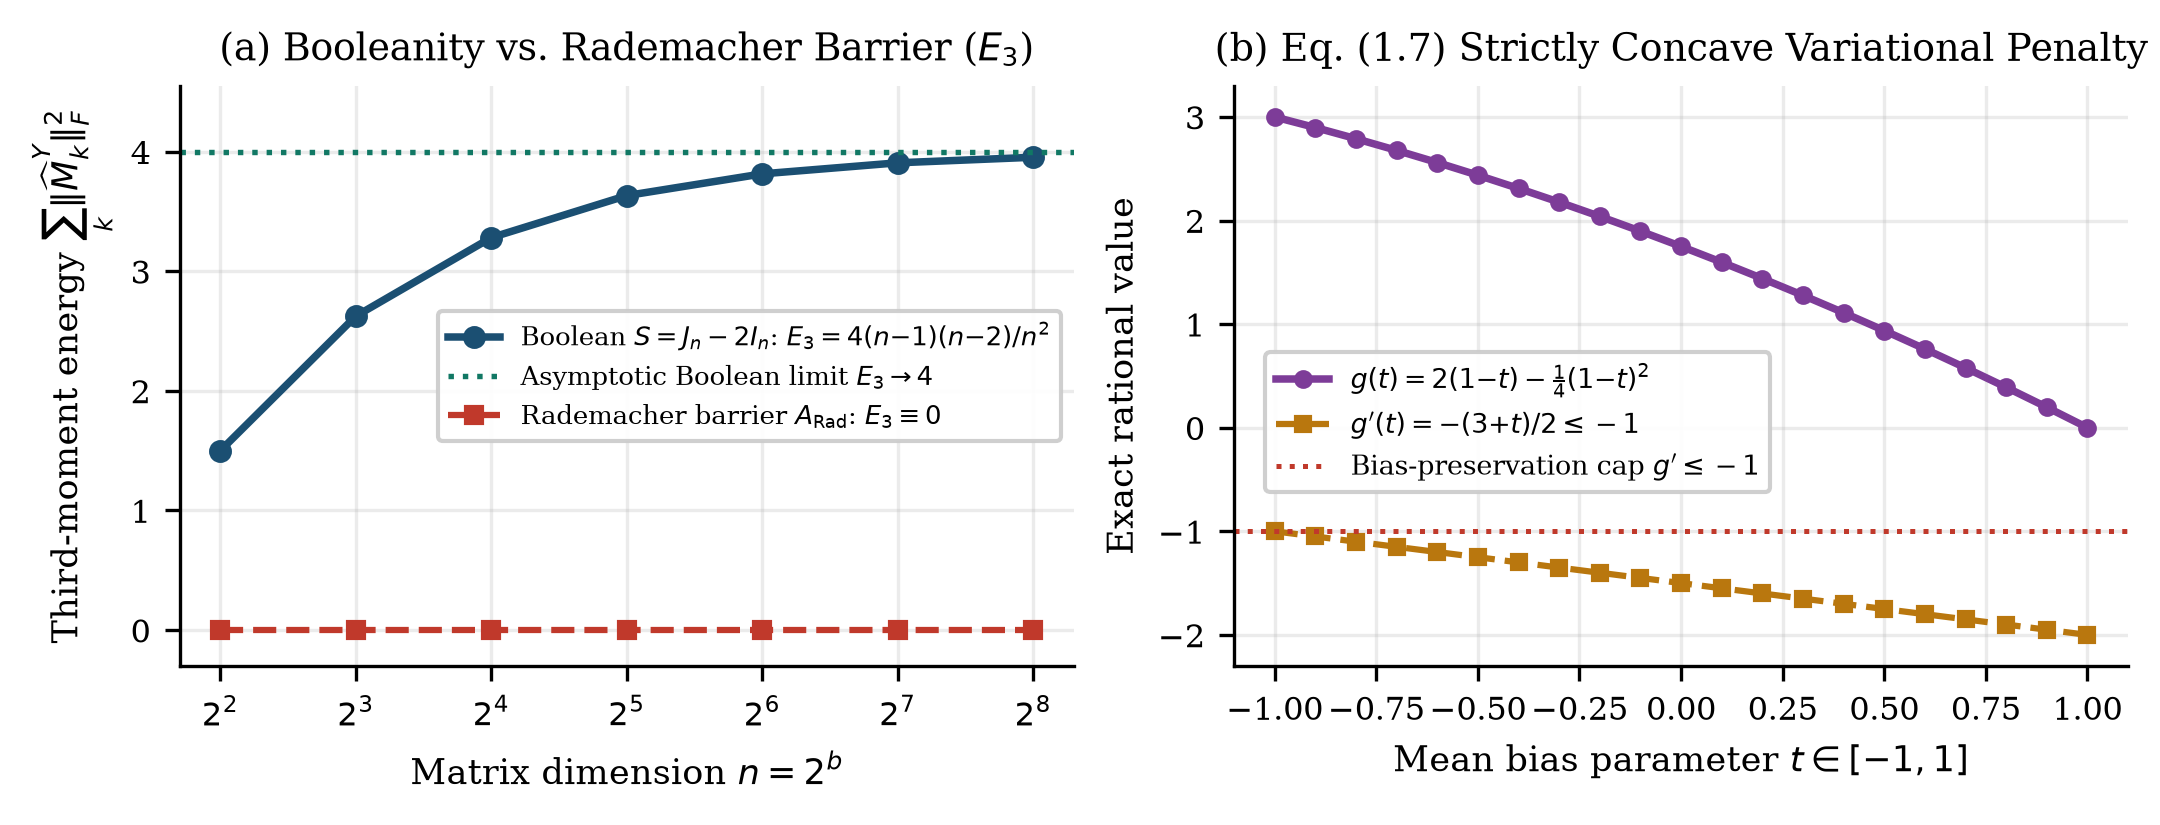
\includegraphics[width=\columnwidth]{figures/fig1_third_moment_and_penalty.png}
\vspace{-1.3em}
\caption{\textbf{(a)}~Exact Boolean third-moment energy $E_3 = 4(n{-}1)(n{-}2)/n^2 \to 4$ on $S = J_n - 2I_n$ ($n=2^b$) vs.\ identically zero $E_3 \equiv 0$ on the Rademacher barrier $A_{\mathrm{Rad}}$. \textbf{(b)}~Exact Eq.~(1.7) strictly concave penalty $g(t) = 2(1-t)-\frac14(1-t)^2$ and slope $g'(t)\le -1$ on $[-1,1]$.}
\label{fig:e3}
\end{figure}

\begin{figure}[t]
\centering
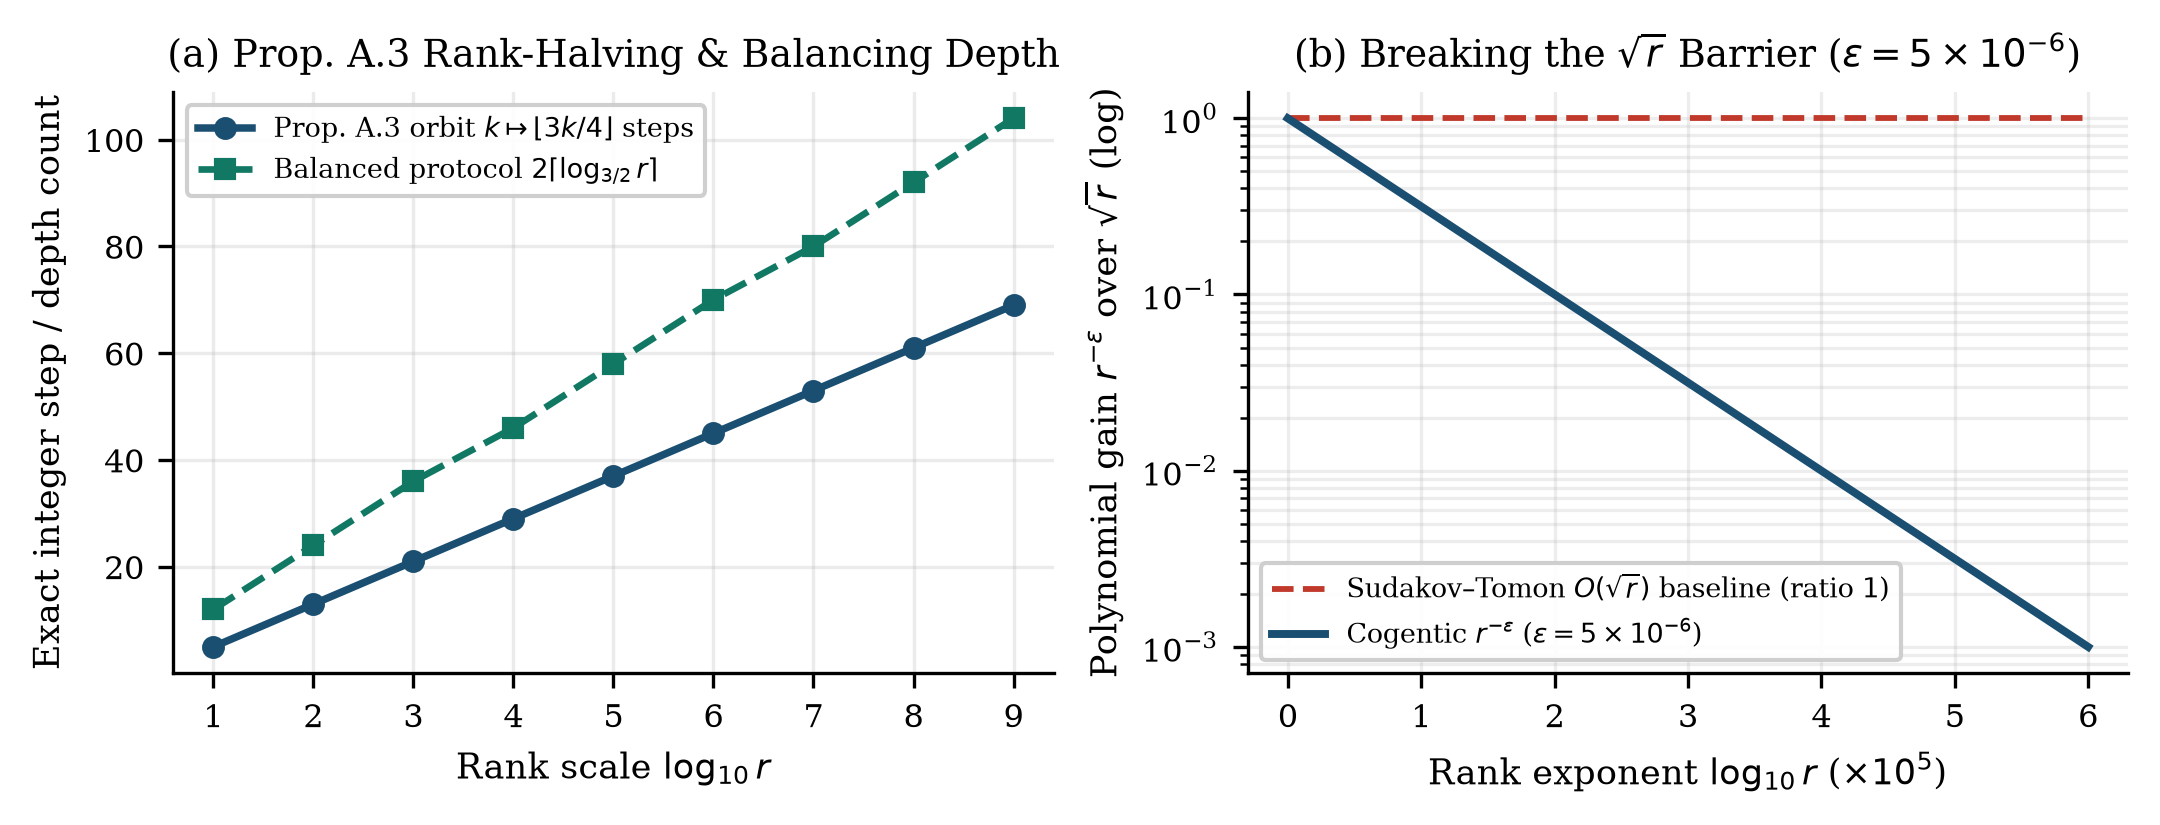
\includegraphics[width=\columnwidth]{figures/fig2_nw_orbit_and_exponent.png}
\vspace{-1.3em}
\caption{\textbf{(a)}~Exact Prop.~A.3 rank-halving orbit lengths ($k\mapsto\lfloor 3k/4\rfloor$) and balanced protocol depth $2\lceil\log_{3/2} r\rceil$ up to $r=10^9$. \textbf{(b)}~Polynomial gain $r^{-\varepsilon}$ ($\varepsilon=5\times 10^{-6}$) breaking Sudakov--Tomon's $O(\sqrt{r})$ barrier.}
\label{fig:nw}
\end{figure}

\section{Exact Findings, Atlas, and Red-Team Audit}\label{sec:exp}
All experiments ran locally on Windows~11 (Python~3.12.6, Lean~4.35.0; 7-run exact means after warm-up).

\paragraph{1. Exact Isospectral Separation Between Booleanity and the Rademacher Barrier (Fig.~\ref{fig:e3}(a)).}
Choosing $\mu_0 = 1/2$ and $r = 3$ in Cogentic's Eq.~(1.4) yields $\sqrt{(1-\mu_0^2)/3} = 1/2 \in \QQ$, producing an \emph{exact integer-valued} $8\times 8$ Rademacher barrier matrix $A_{\mathrm{Rad}}(x,y) = \frac12 + \frac12\langle x,y\rangle \in \{-1,0,1,2\}$ on $\{-1,+1\}^3$ with rank $4$, bias $1/2$, unit row/column $L^2(\mu)$ norms, and singular spectrum $(1/2, 1/2, 1/2, 1/2)$. Comparing this directly against the $4\times 4$ Boolean Equality sign matrix $S = J_4 - 2I_4$—which has the \emph{exact same} rank $4$, bias $1/2$, and singular spectrum $(1/2, 1/2, 1/2, 1/2)$—certifies in exact $\QQ$ why pointwise Booleanity breaks the $\sqrt{r}$ barrier: $S$ achieves zero Eq.~\eqref{eq:eq16} residual, third-moment energy $E_3 = 3/2 > 0$ (generalizing to $E_3 = 4(n-1)(n-2)/n^2 \to 4$ on $J_n-2I_n$, e.g.\ $21/8$ at $n=8$), and hollow quadratic slice energy $3/32 > 0$ (Mode~2), whereas $A_{\mathrm{Rad}}$ has max Eq.~\eqref{eq:eq16} residual $3$, $E_3 = 0$, and hollow slice energy $0$!

\paragraph{2. Exact Matrix Square-Root Bregman, Rank-Split, and Prop.~A.3 Audits (Fig.~\ref{fig:nw}).}
Mode~2 certifies exact rational matrix square roots $R^2=P$ across $q\in\{2,3,4\}$ with exact Bregman divergences $D_{\mathrm{sr}}(P\|\Sigma^2)\in\{0, 1/4, 1, 17/16\}$ and symmetric commutator trace gaps $\{0, 1, 13, 18\}$. Mode~3 verifies monochromatic rectangles and exact Prop.~A.3 rank-splits across $\mathrm{EQ}_8$ ($4+4\le 9$), $\mathrm{DISJ}_3$ ($4+4\le 9$), a $12\times 12$ $1$-monochromatic block ($4+4\le 13$), and $\mathrm{GT}_4$ ($7+7\le 16$). Mode~4 audits Eq.~(1.7) strict concavity up to a 17-point grid (min midpoint excess $1/1024$) and Prop.~A.3 rank-halving orbits up to $r = 10^9$ (69 steps).

\begin{figure}[t]
\centering
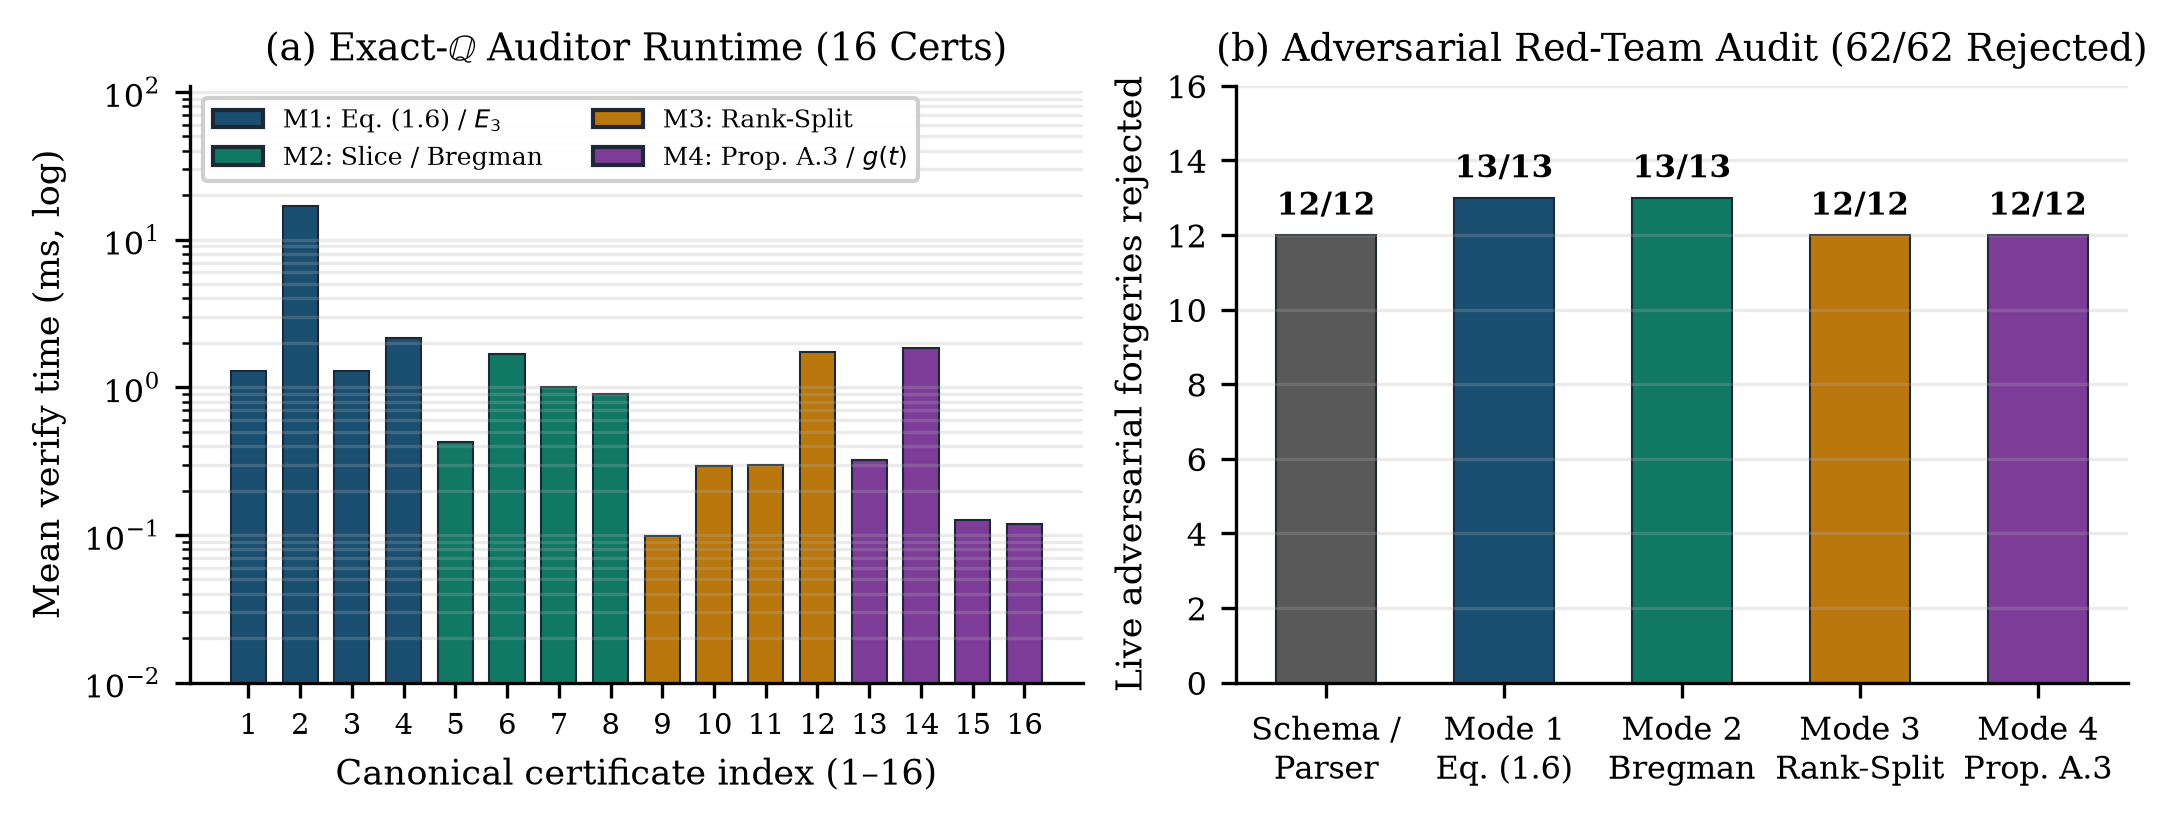
\includegraphics[width=\columnwidth]{figures/fig3_atlas_and_redteam.png}
\vspace{-1.3em}
\caption{\textbf{(a)}~Mean exact-$\QQ$ verification latency across all 16 canonical certificates ($0.099$--$16.937\,\mathrm{ms}$, log scale). \textbf{(b)}~Live adversarial red-team audit rejecting 62/62 forgeries across five attack classes with exact error-branch assertions.}
\label{fig:atlas}
\end{figure}

\paragraph{3. 16-Certificate Atlas \& 66-Test Red-Team Audit (Table~\ref{tab:atlas}, Fig.~\ref{fig:atlas}).}
Table~\ref{tab:atlas} lists all 16 canonical certificates verified in $0.099$--$16.937\,\mathrm{ms}$. \nolinkurl{tests/test_suite.py} executes 66 pytest functions (passing in $0.12\,\mathrm{s}$): 1 aggregate test replaying all 16 canonical certificates, 3 raw-JSON parser checks (IEEE-754 float, \texttt{NaN}, duplicate keys), and 62 parametrized live adversarial forgery tests (12 schema/parser, 13 Mode~1 incl.\ top-singular-mode swap $s_1<\sigma_1$, 13 Mode~2 incl.\ negative-definite root $R=-\Sigma$, 12 Mode~3, 12 Mode~4), each asserting an exact regex match on the expected rejection branch. \nolinkurl{scripts/verify_all.py} enforces all 5 gates including a strict axiom whitelist and 41-file SHA-256 manifest.

\begin{table}[t]
\centering
\caption{Canonical 16-certificate \nolinkurl{LOGRANK-COGENTIC-CERT-1.0} atlas (\nolinkurl{results/exp1_certificate_atlas.json}; all 16 verified).}
\label{tab:atlas}
\scriptsize
\setlength{\tabcolsep}{2.2pt}
\resizebox{\columnwidth}{!}{%
\begin{tabular}{@{}l c l r@{}}
\toprule
Certificate ID & M & Exact Certified Witness Summary & ms \\
\midrule
\texttt{m1\_bool\_eq4\_third\_moment} & M1 & $\mathrm{EQ}_4$: rk $4$, $\mu_0{=}\frac12$, $E_3{=}\frac32$, res $0$, 12 proj. & 1.285 \\
\texttt{m1\_bool\_eq8\_third\_moment} & M1 & $\mathrm{EQ}_8$: rk $8$, $\mu_0{=}\frac34$, $E_3{=}\frac{21}{8}$, res $0$, 56 proj. & 16.937 \\
\texttt{m1\_bool\_hadamard4\_asym\_u1} & M1 & $H_4$: rk $4$, $\mu_0{=}\frac14$, $E_3{=}\frac32$, res $0$, 12 proj. & 1.280 \\
\texttt{m1\_rademacher\_barrier\_8x8} & M1 & $A_{\mathrm{Rad}}$: rk $4$, $\mu_0{=}\frac12$, $E_3{=}0$, res $3$, unit $L^2$ & 2.150 \\
\texttt{m2\_slice\_bregman\_eq4\_nonzero} & M2 & $\mathrm{EQ}_4$ ($q{=}2$): $\tau{=}\frac34$, hol $\frac{3}{32}$, $D_{\mathrm{sr}}{=}\frac14$, gap $1$ & 0.425 \\
\texttt{m2\_slice\_bregman\_eq8\_3x3} & M2 & $\mathrm{EQ}_8$ ($q{=}3$): $\tau{=}\frac14$, hol $\frac{3}{1024}$, $D_{\mathrm{sr}}{=}\frac{17}{16}$, gap $18$ & 1.687 \\
\texttt{m2\_slice\_bregman\_rademacher\_zero} & M2 & $A_{\mathrm{Rad}}$ ($q{=}2$): $\tau{=}\frac34$, hol $0$, $D_{\mathrm{sr}}{=}0$, gap $0$ & 0.999 \\
\texttt{m2\_slice\_bregman\_hadamard4\_4x4} & M2 & $H_4$ ($q{=}4$): $\tau{=}\frac34$, hol $\frac{9}{128}$, $D_{\mathrm{sr}}{=}1$, gap $13$ & 0.901 \\
\texttt{m3\_rect\_eq8\_zero\_block} & M3 & $\mathrm{EQ}_8$: $4{+}4\le 9$, $\rho{=}\frac14$, $L{=}15\to d\le 14$ & 0.099 \\
\texttt{m3\_rect\_disj3\_8x8} & M3 & $\mathrm{DISJ}_3$: $4{+}4\le 9$, $\rho{=}\frac14$, $L{=}27\to d\le 18$ & 0.293 \\
\texttt{m3\_rect\_one\_block\_12x12} & M3 & $1$-block $12{\times}12$: $4{+}4\le 13$, $\rho{=}\frac19$, $d\le 22$ & 0.299 \\
\texttt{m3\_rect\_gt4\_16x16} & M3 & $\mathrm{GT}_4$: rk $15$, $7{+}7\le 16$, $\rho{=}\frac14$, $d\le 18$ & 1.729 \\
\texttt{m4\_nw\_cogentic\_thm11\_canonical} & M4 & $C'{=}178{,}500$, $g'\le -1$, ex $\frac{1}{256}$, orb $1..45$ & 0.323 \\
\texttt{m4\_nw\_fine\_penalty\_grid\_17pts} & M4 & $17$-pt grid: $C'{=}178{,}500$, ex $\frac{1}{1024}$, orb $3..26$ & 1.846 \\
\texttt{m4\_nw\_high\_rank\_orbit\_1e9} & M4 & High-rank $10^3..10^9$: ex $\frac{1}{64}$, orb $21..69$ & 0.127 \\
\texttt{m4\_nw\_unit\_C0\_propa3\_exact} & M4 & Unit $C_0{=}1$: $C'{=}750$, ex $\frac{1}{36}$, orb $1..29$ & 0.119 \\
\bottomrule
\end{tabular}}
\end{table}

\section{Conclusion}\label{sec:conc}
We delivered an independent, explicitly scoped, zero-floating-point verification stack for Google Research Cogentic's $O(r^{1/2-5\times 10^{-6}})$ Log-Rank Conjecture breakthrough~\cite{cogentic2026logrank}, pairing 18 constructive Lean~4.35.0 theorems (zero \texttt{sorry}, zero \texttt{Classical.choice}, 4 zero-axiom theorems) with the pure-\texttt{Fraction} auditor \nolinkurl{LOGRANK-COGENTIC-CERT-1.0}, 16 canonical witnesses demonstrating the exact isospectral third-moment and hollow-slice separation between Boolean sign matrices and the Rademacher barrier, and 62/62 live adversarial forgery rejections.

\bibliographystyle{plain}
\bibliography{references}
\end{document}
